\section{导数的概念}
\subsection{导数的定义}
\begin{example}
求曲线$y=f(x)$在曲线上的点$ \left( x_0,y_0 \right)$处切线的斜率。
\end{example}
\begin{center}
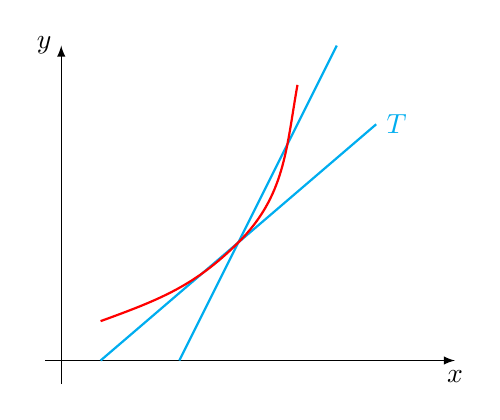
\begin{tikzpicture}
%\draw[help lines] (0,0) grid (5,4);
\draw[->,>=latex] (-0.2,0)--(5,0) node[below] {$x$};
\draw[->,>=latex] (0,-0.3)--(0,4) node[left] {$y$};
\draw[cyan,thick] (0.5,0)--(4,3) node[right] {$T$};
\draw[cyan,thick] (1.5,0)--(3.5,4);
\draw[thick,red] (0.5,0.5)to [out=20,in=225] (2.25,1.5);
\draw[thick,red] (2.25,1.5) to [out=45,in=260] (3,3.5);
\end{tikzpicture}
\end{center}
在曲线$y=f(x)$上点$P_0(x_0,y_0)$的附近另取一点$P_1(x,y)$,连接$P_1$和$P_0$得割线$P_0P_1$,当$P_1$沿曲线趋于$P_0$时,割线$P_0P_1$的极限位置称为曲线在点$P_0$的切线。
令$x=x_0+\Delta x,y=y_0+\Delta y$,则$P_0P_1$的斜率为$\dfrac{\Delta y}{\Delta x}$,如果$$ \lim_{\Delta x\rightarrow 0} \dfrac{\Delta y}{\Delta x}=\lim_{\Delta x\rightarrow 0} \dfrac{f(x_0+\Delta x-f(x_0))}{\Delta x}$$
存在,则此极限值就是曲线的切线的斜率。
设切线的倾角为$\alpha$,则$$\tan \alpha=\lim_{\Delta x\rightarrow 0} \dfrac{f(x_0+\Delta x)-f(x_0)}{\Delta x}$$ 
从另一角度,$\dfrac{\Delta y}{\Delta x}$表示$y=f(x)$在区间$\left[~x_0,x_0+\Delta x\right]$(或$\left[~x_0+\Delta x,x_0\right]$)的平均变化率,极限$\lim\limits_{\Delta x\rightarrow 0} \dfrac{\Delta y}{\Delta x}$称为函数$f(x)$在$x_0$的变化率。
\begin{example}
求变速直线运动的物体的瞬时速度。物体产生的位移$s$是时间$t$的函数,设运动方程为$s=s(t)$,求在$t_0$时刻的速度。
\end{example}
\begin{solution}
\[\dfrac{\Delta s}{\Delta t}=\dfrac{s(t_0+\Delta t)-s(t_0)}{\Delta t} \]
\[ v(t_0)=\lim_{\Delta t\rightarrow 0} \dfrac{\Delta s}{\Delta t}=\lim_{\Delta t\rightarrow 0} \dfrac{s(t_0+\Delta t)-s(t_0)}{\Delta t} \].
\end{solution}
\begin{description}
\item[{\kaishu \zihao{4}\hspace{2em}\color{cyan}\ding{229}定义}]\hspace{1.5em}设函数$y=f(x)$在点$x_0$的邻域内有定义,当自变量$x$从$x_0$变到$x_0+\Delta x$时,则函数得相应的增量$\Delta y=f(x_0+\Delta x)-f(x_0)$,如果极限$$\lim_{\Delta x\rightarrow 0} \dfrac{\Delta y}{\Delta x}=\lim_{\Delta x\rightarrow 0} \dfrac{f(x_0+\Delta x)-f(x_0)}{\Delta x}$$存在,则称函数$y=f(x)$在点$x_0$可导,并称此极限为函数$f(x)$在点$x_0$的导数。记作$f^\prime (x_0)$,或$y^\prime (x_0),\ y^\prime|_{x=x_0},\ \dfrac{dy}{dx}\left|_{x=x_0}\right.,\ \dfrac{df(x)}{dx}\left|_{x=x_0}\right.$~.即:$$f^\prime (x_0)=\lim_{\Delta x\rightarrow 0} \dfrac{\Delta y}{\Delta x}=\lim_{\Delta x\rightarrow 0} \dfrac{f(x_0+\Delta x)-f(x_0)}{\Delta x}.$$
\end{description}
如果记$x_0+\Delta x=x$,则上式可写为$$f^\prime (x_0)=\lim_{x\rightarrow x_0} \dfrac{f(x)-f(x_0)}{x-x_0} %
\text{或记}h=\Delta x,$$则$f^\prime (x_0)=\lim_{h\rightarrow 0} \dfrac{f(x_0+h)-f(x_0)}{h},$%
如果上述极限不存在,则称函数在点$x_0$不可导。
\begin{example}
设$y=f(x)$在$x_0$处可导\begin{enumerate}[(1)]
\item $\lim\limits_{h\rightarrow 0} \dfrac{f(x_0+h)-f(x_0-h)}{h}=?$ 
\item $\lim\limits_{\Delta x\rightarrow 0} \dfrac{f(x_0+2\Delta x)-f(x_0)}{\Delta x}=1$,则$f^\prime (x_0)=?$
\end{enumerate}
\vspace{-5mm}
\end{example}
\begin{solution}
$(1)\lim_{h\rightarrow 0}\dfrac{f(x_0+h)-f(x_0-h)}{h} \\=\lim_{h\rightarrow 0} \dfrac{f(x_0+h)-f(x_0)+f(x_0)-f(x_0-h)}{h} \\=\lim_{h\rightarrow 0} \dfrac{f(x_0+h)-f(x_0)}{h}+\lim_{h\rightarrow 0} \dfrac{f(x_0-h)-f(x_0)}{-h} \\=2f^\prime (x_0).\\
 (2)\lim\limits_{\Delta x\rightarrow 0} \dfrac{f(x_0+2\Delta x)-f(x_0)}{\Delta x}\\=2\lim\limits_{\Delta x\rightarrow 0} \dfrac{f(x_0+2\Delta x)-f(x_0)}{2\Delta x}\\=2f^\prime (x_0)=1\\
 \therefore f^\prime (x_0)=\dfrac{1}{2}$
\end{solution}
\begin{example}
设$f^\prime (x_0)=5$,且$\lim\limits_{\Delta x\rightarrow 0} \dfrac{f(x_0)-f(x_0-k\Delta x)}{\Delta x}=-10$,则$k=$?
\end{example}
\begin{solution}
$\lim\limits_{\Delta x\rightarrow 0} \dfrac{f(x_0)-f(x_0-k\Delta x)}{\Delta x}\\=k\lim\limits_{\Delta x\rightarrow 0} \dfrac{f(x_0-k\Delta x)-f(x_0)}{-k\Delta x}\\=kf^\prime (x_0)=5k=-10\\ \therefore k=-2$
\end{solution}
\begin{example}
证明:$y=\sqrt[3]{x}$在$x=0$处不可导。
\end{example}
\begin{solution}
$\lim\limits_{\Delta x\rightarrow 0} \dfrac{f(x)-f(0)}{x-0}=\lim\limits_{x\rightarrow 0} \dfrac{\sqrt[3]{x}}{x}=\lim\limits_{x\rightarrow 0} \dfrac{1}{\sqrt[3]{x^2}}=\infty \\\therefore y=\sqrt[3]{x} \text{在}x=0\text{处不可导。}$
\end{solution} 
{\kaishu \color{blue}注意:函数$y=\sqrt[3]{x}$在$(0,0)$处的切线存在,斜\\
率为$\infty$,所以函数$f(x)$在$x_0$处有$\lim\limits_{\Delta x\rightarrow 0} \dfrac{\Delta y}{\Delta x}=\infty$或\\
$\lim\limits_{x\rightarrow x_0} \dfrac{f(x)-f(x_0)}{x-x_0}=\infty$时,有时也称$f(x)$在$x_0$处导\\
数无穷大。
}
\vspace{-3.5cm}
\begin{flushright}
\begin{tikzpicture}
\draw[->,>=latex] (-3.2,0)--(3.2,0) node[below] {$x$};
\draw[->,>=latex] (0,-1.5)--(0,1.5) node[left] {$y$};
\draw [domain=0:3,samples=1000,cyan] plot(\x,{(\x)^(1/3)}) node[above] {$y=\sqrt[3]{x}$};
\draw [domain=-3:0,samples=1000,cyan] plot(\x,{-(-\x)^(1/3)});
\coordinate [label=below right:$O$](o) at (0,0);
\end{tikzpicture}
\end{flushright}
\begin{example}
讨论函数$f(x)=\Bigg\{\begin{aligned}
&\ln \left(1+x\right),&-1<x\leq 0\\
&\sin x,&x>0\\
\end{aligned}$在$x=0$处的可导性。
\end{example}
\begin{solution}
$f(0)=0  \\
f^\prime_{-}(0)=\lim\limits_{x\rightarrow 0^{-}} \dfrac{f(x)-f(0)}{x-0}=\lim\limits_{x\rightarrow 0^{-}} \dfrac{\ln\left(1+x\right)-0}{x}=1 \\
f^\prime_{+}(0)=\lim\limits_{x\rightarrow 0^{+}} \dfrac{f(x)-f(0)}{x-0}=\lim\limits_{x\rightarrow 0^{+}} \dfrac{\sin x-0}{x}=1 \\
\therefore f(x)\text{在}x=0\text{可导且}f^\prime (0)=1.$
\end{solution}
如果函数$f(x)$在区间$I$内每一点都可导(闭区间时,左端点须右可导,右端点须左可导),则称函数$f(x)$在区间$I$内可导,此时其导数值是随$x$而变的函数,称为$f(x)$的导函数,简称导数,记作$$f^\prime (x),~y^\prime,~\dfrac{df(x)}{dx},~\dfrac{dy}{dx}.$$ 
而$f^\prime (x_0)$是$f(x)$的导函数$f^\prime (x)$在$x=x_0$处的函数值。

{\kaishu \hspace{-2em}\color{cyan}\ding{45}~~总结:用定义求函数的导数(函数),可分三步进行:
\begin{enumerate}[1)]
\item 求增量$\Delta y=f(x+\Delta x)-f(x)$
\item 求比值$\dfrac{\Delta y}{\Delta x}=\dfrac{f(x+\Delta x)-f(x)}{\Delta x}$
\item 求极限$\lim\limits_{\Delta x\rightarrow 0}\dfrac{\Delta y}{\Delta x}$
\end{enumerate}}
\begin{example}
求$y=x^n$($n$为正整数)
\end{example}
\begin{solution}
$\Delta y=(x+\Delta x)^n-x^n~~~\text{应用二项式定理} \\
=x^n+nx^{n-1}\Delta x+\dfrac{n(n-1)}{2!} x^{n-2}(\Delta x)^2+\cdots+(\Delta x)^n-x^n \\
=nx^{n-1}\Delta x+\dfrac{n(n-1)}{2!}x^{n-2}(\Delta x)^2+\cdots+(\Delta x)^n \\
\dfrac{\Delta y}{\Delta x}=nx^{n-1}+\dfrac{n(n-1)}{2!}x^{n-2}\Delta x+\cdots+(\Delta x)^{n-1}   \\ \lim\limits_{\Delta x\rightarrow 0}\dfrac{\Delta y}{\Delta x}=nx^{n-1},\text{所以}(x^n)^\prime=nx^{n-1}~$
\end{solution}

{\kaishu \color{blue}一般有:$\left(x^{~\mu}\right)^\prime=\mu x^{~\mu-1},\mu$为任意实数。}
\par 
利用导数的定义和基本求导法则求出了常用初等函数的导数:
\begin{center}
\begin{tabular}{|c|c|c|c|}
\hline
$(c)^\prime=0$&$(x^{~\mu})^\prime=\alpha x^{~{\mu-1}}$&$(\sin x)^\prime=\cos x$&
$(\cos x)^\prime=-\sin x$ \\ 
\hline
$(\tan x)^\prime=\sec^2 x$&$(\cot x)^\prime=-\csc^2 x$&$(\sec x)^\prime=\sec x\tan x$&$(\csc x)^\prime=-\csc x\cot x$ \\
\hline
$\Gape[10pt] (a^x)^\prime=a^x \ln x$&$(\mathrm{e}^x)^\prime=\mathrm{e}^x$&$(\log_a x)^\prime=\dfrac{1}{x \ln a}$&$(\ln x)^\prime=\dfrac{1}{x}$ \\
\hline
$\Gape[10pt] (\arcsin x)^\prime=\dfrac{1}{\sqrt{1-x^2}}$&$(\arccos x)^\prime=-\dfrac{1}{\sqrt{1-x^2}}$&$(\arctan x)^\prime=\dfrac{1}{1+x^2}$&$(\mathrm{arccot}~x)^\prime=-\dfrac{1}{1+x^2}$  \\
\hline
\end{tabular}
\end{center}
\begin{example}
设$y=x^3 \sqrt{x}$~,求$y^\prime~,y^\prime|_{x=1}$~.
\end{example}
\begin{solution}
$y=x^{\frac{7}{2}}~,y^\prime=\dfrac{7}{2} x^{\frac{5}{2}}~,y^\prime|_{x=1}=\dfrac{7}{2}$~.
\end{solution}
\subsection{可导与连续的关系}
\begin{description}
\item[{\kaishu \zihao{4}\hspace{2em}\color{cyan}\ding{229}定理}]\hspace{1.5em}如果函数$y=f(x)$在点$x$可导,则函数$y=f(x)$在点$x$连续。
\end{description}
因为$f(x)$在点$x$可导,即$\lim\limits_{\Delta x\rightarrow 0} \dfrac{\Delta y}{\Delta x}=\lim\limits_{\Delta x\rightarrow 0}\dfrac{f(x+\Delta x)-f(x)}{\Delta x}=f^\prime(x), \\
\therefore \dfrac{\Delta y}{\Delta x}=f^\prime(x)+\alpha\left(\Delta x\right),\\
\Delta y=f^\prime(x)\Delta x+o\left(\Delta x\right) \text{(增量公式)} \\
\text{即}\Delta y=f(x+\Delta x)-f(x)=f^\prime(x)\Delta x+o\left(\Delta x\right) \\
\text{所以}\Delta x\rightarrow 0\text{时},\Delta y\rightarrow 0.f(x)\text{在}x\text{处连续}.$\\
{\kaishu \color{blue}注:定理的逆不一定成立,即函数$y=f(x)$在点$x$连续,却不一定可导。}


\begin{example}
函数$y=f(x)=\abs{x}$,在点$x=0$连续,但不可导。
\end{example}
\begin{solution}
$\because y=f(x)=\abs{x}=\Bigg\{\begin{aligned}
&x,&x\geq 0, \\
&-x,&x<0. \\
\end{aligned}$
\begin{center}
\begin{tikzpicture}
\draw[->,>=latex] (-2,0)--(2,0) node[below] {$x$};
\draw[->,>=latex] (0,-0.5)--(0,2.5) node[left] {$y$};
\draw [domain=-1.6:1.6,samples=1000,cyan] plot(\x,{abs(\x)}) node[above] {$y=\abs{x}$};
\coordinate [label=below left:$O$](o) at (0,0);
\end{tikzpicture}
\end{center}
$\lim\limits_{n\rightarrow 0^{-}}f(x)=\lim\limits_{n\rightarrow 0^{+}}f(x)=0=f(0)$~,所以$y=\abs{x}$在$x=0$连续。\\
$\dfrac{\Delta y}{\Delta x}=\dfrac{f(0+\Delta x)-f(0)}{\Delta x}=\dfrac{\left|~\Delta x~\right|}{\Delta x}=\Bigg\{\begin{aligned}
&~1,&\Delta x>0,
&~-1,&\Delta x<0,
\end{aligned} \\
\therefore f_{+}^\prime(0)=1,f_{-}^\prime(0)=-1,y=\abs{x}\text{在}x=0\text{不可导}.$
\end{solution}
\begin{example}
讨论函数$f(x)=\Bigg\{\begin{aligned}
&x^2 \dfrac{1}{\sin x},&x\neq 0 \\
&0,&x=0 \\
\end{aligned}$在$x=0$处的连续性与可导性。
\end{example}
\begin{solution}
$\because \lim\limits_{x\rightarrow 0} f(x)=\lim\limits_{x\rightarrow 0}x^2 \sin \dfrac{1}{x}=0=f(0), \therefore f(x)\text{在}x=0\text{处连续。}\\
\lim\limits_{x\rightarrow 0}\dfrac{f(x)-f(0)}{x-0}=\lim\limits_{x\rightarrow 0}\dfrac{x^2 \sin \dfrac{1}{x}}{x}=\lim\limits_{x\rightarrow 0}x \sin \dfrac{1}{x}=0 \\
\therefore f(x)\text{在}x=0\text{处可导,且}f^\prime(0)=0.$
\end{solution}
\begin{example}
设$f(x)=\Bigg\{\begin{aligned}
&e^x ,&x< 0 \\
&a+bx,&\geq 0 \\
\end{aligned}$问当$a,b$为何值时,$f(x)$在$x=0$连续且可导。
\end{example}
\begin{solution}
$f(x)$在$x=0$处连续,则$f(0)=\lim\limits_{x\rightarrow 0^{-}}f(x)=\lim\limits_{x\rightarrow 0^{+}}f(x)$~,\\$\therefore a=1$~\\$f_{-}^\prime(0)=\lim\limits_{x\rightarrow 0^{-}}\dfrac{f(x)-f(0)}{x-0}=\lim\limits_{x\rightarrow 0^{-}}\dfrac{e^x-1}{x}=1$~\\
$f_{+}^\prime(0)=\lim\limits_{x\rightarrow 0^{+}}\dfrac{f(x)-f(0)}{x-0}=\lim\limits_{x\rightarrow 0^{+}}\dfrac{(1+bx)-1}{x}=b$~\\
$f(x)$在$x=0$处可导,则$f_{-}^\prime(0)=f_{+}^\prime(0),~~\therefore b=1$
\end{solution}
\subsection{导数的几何意义}
\begin{center}
\begin{tikzpicture}
\tikzmath{
\a=sqrt(3);
}
\draw[->,>=latex] (-0.2,0)--(4,0) node[below] {$x$};
\draw[->,>=latex] (0,-0.2)--(0,3) node[left] {$y$};
\draw[thick,cyan] (0.5,0)--(3.5,\a) node[right] {$T$};
\draw[thick,blue] (0.8,1.1) parabola bend (2,1) (3.5,2.4) node[left] {$y=f(x)$};
\draw[dashed] (2.5,0) node[below] {$x_0$}--(2.5,1.2) node[left] {$M$};
\node[below left] at (0,0) {$O$};
\draw (1,0) arc (0:15:1);
\node at (8:1.2) {$\alpha$};
\end{tikzpicture}
\end{center}
\begin{description}
\item[{\kaishu \zihao{4}\hspace{2em}\color{cyan}\ding{229}导数的几何意义}]\hspace{1.5em}$y=f(x)$在点$x_0$的导数$f^\prime (x_0)$是曲线$y=f(x)$在点$M(x_0,y_0)$处切线的斜率。
所以$y=f(x)$在$(x_0,y_0)$处的切线方程为$$y-y_0=f^\prime (x_0)(x-x_0)$$法线方程为$$y-y_0=\dfrac{-1}{f^\prime (x_0)}(x-x_0)$$
\end{description}
\begin{example}
求$y=x^2$在$(-1,1)$处的切线方程和法线方程。
\end{example}
\begin{solution}
$y^\prime 2x,~y^\prime (-1)=-2 \\
\text{切线方程为}y-1=-2\left[~x-(-1)\right],\text{即}2x+y+1=0 \\
\text{法线方程为}y-1=-\dfrac{1}{-2}\left[~x-(-1)\right],\text{即}x-2y+3=0.$
\end{solution}
\begin{example}
设曲线$y=2x+\ln x$上的点$M(x_0,y_0)$处的切线平行于直线$y=4x$,求点$M$的坐标。
\end{example}
\begin{solution}
$y^\prime =2+\dfrac{1}{x}$~,因为曲线在$M$点的切线平行于$y=4x$,\\
$\therefore y^\prime(x_0)=2+\dfrac{1}{x_0}=4$ \\
解出$x_0=\dfrac{1}{2},y_0=2x_0+\ln x_0=1+\ln \dfrac{1}{2}=1-\ln 2$ \\
所以$M$点的坐标为$\left(~\dfrac{1}{2},1-\ln 2\right)$~。
\end{solution}
